\documentclass[11pt]{article}

\usepackage{adb}

\newcommand{\mybox}{%
    \collectbox{%
        \setlength{\fboxsep}{4pt}%
        \fbox{\BOXCONTENT}%
    }%
}

\oddsidemargin0cm
\topmargin-2cm     %I recommend adding these three lines to increase the 
\textwidth16.5cm   %amount of usable space on the page (and save trees)
\textheight23.5cm  
\newcommand{\question}[1] {\vspace{.3in} \hrule\vspace{0.3em}
\noindent{\bf #1} \vspace{0.7em}
\hrule \vspace{.10in}}
\renewcommand{\part}[1] {\vspace{.10in} {\bf (#1)}}

\newcommand{\myinfo}{Albert Gao / sixiangg}
\newcommand{\myhwnum}{1}
\newcommand{\currdate}{04/05/2022}

\newcommand{\Gen}{\textsf{Gen}}
\newcommand{\Eval}{\textsf{Eval}}
\newcommand{\Agg}{\textsf{Agg}}
\newcommand{\Rec}{\textsf{Rec}}
\newcommand{\Sim}{\textsf{Sim}}
\newcommand{\Real}{\textsf{Real}}
\newcommand{\Ideal}{\textsf{Ideal}}

\setlength{\parindent}{0pt}
\setlength{\parskip}{5pt plus 1pt}
 
%\pagestyle{fancyplain}
%\lhead{\fancyplain{}{\textbf{HW\myhwnum}}}      % Note the different brackets!
%\rhead{\fancyplain{}{\bigskip\myinfo}}
%\chead{\fancyplain{}{21-623}}

\begin{document}

\bigskip                        % Skip a "medium" amount of space
                                % (latex determines what medium is)
                                % Also try: \bigskip, \littleskip

\thispagestyle{plain}
\begin{center}                  % Center the following lines
{\Huge DPF Using Learning With Errors}

\vspace{0.3cm}

\large{\myinfo}

\large{\currdate}

\end{center}

\section{Context}
Again, we explore the problem of PIR and the problem of DPF. We attempt to show that existing techniques in homomorphic encryption based on learning with errors (LWE) assumptions suffice to give a solution to PIR and to DPF. Specifically, if there is one server with a database of $n$ items, then PIR can be done using $O(\text{polylog}(n))$ communication complexity and $\widetilde{O}(n)$ computation complexity on server side. Further, for our purposes, due to relative simplicity of circuits we evaluate, we can refrain from using fully homomorphic encryption and, for example, opt for somewhat/leveled homomorphic encryption without the so-called ``bootstrapping'' technique. In other words, this approach can be made practically feasible without relying on fully homomorphic encryption. 

Extension from one-server PIR to the multi-server DPF setting is simple and uninteresting: perform exactly the same method for each server. This should tolerate collusion among all servers and/or failures from all but one servers. Indeed, this method sounds degenerate enough for the DPF setting that it makes replication of data on different servers unappealing for our purposes. However, 
the asymptotic or concrete complexity from this note can still serve as a benchmark for other DPF approaches.

\section{Prelim}
To keep it consistent, all relevant techniques in this section can be found in~\cite{halevi17}. We provide a summary of the ones we need for our purposes.
\subsection{Warmup}
Homomorphic encryption involves computation on encrypted data. In our informal mental model, to evaluate a circuit on some plaintext inputs, we may also equivalently evaluate some procedure (that is based on this circuit) on inputs consisting of encrypted bits, and the resulting new ciphertext can be decrypted to the plaintext result we desire. An uninteresting approach to this problem can simply attach the original circuit to the ciphertext inputs and call it the new ciphertext. The decryption procedure would simply decrypt each of the ciphertext inputs and evaluate the attached circuit. In order to capture the notion of having a similar decryption procedure between ``freshly generated'' ciphertexts and ``evaluated'' ciphertexts, we need the nontrivial notion of \textit{compactness} for our homomorphic encryption schemes, where complexity of decryption does not depend on the complexity of the circuit we evaluate.

Without specifying precise definitions of homomorphic encryption and compactness, we can still see that this can be used for PIR assuming constructions are feasible. A server can evaluate a circuit for the function $f_{db}(i) = db[i]$ using homomorphic encryption, where the database consisting of $n$ items is hardwired in the circuit and the interested index $i$ is encrypted before reaching the server. An example circuit with a database $(1,0,1,1) \in \{0,1\}^4$ and index bits $a,b$ is illustrated in Figure~\ref{fig:fig1}. It is clear that homomorphic encryption should give us desired output if the server is given encrypted versions of $a, \lnot a, b, \lnot b$. One more important observation here is that the depth of this circuit before the last degree-$n$ fan-in gate is exactly $\lceil \log n \rceil$. From a different perspective, we are computing the sum of $n$ bits, each of which is the result of $\lceil \log n \rceil$ multiplications. 

\begin{figure}[h]
  \centering
  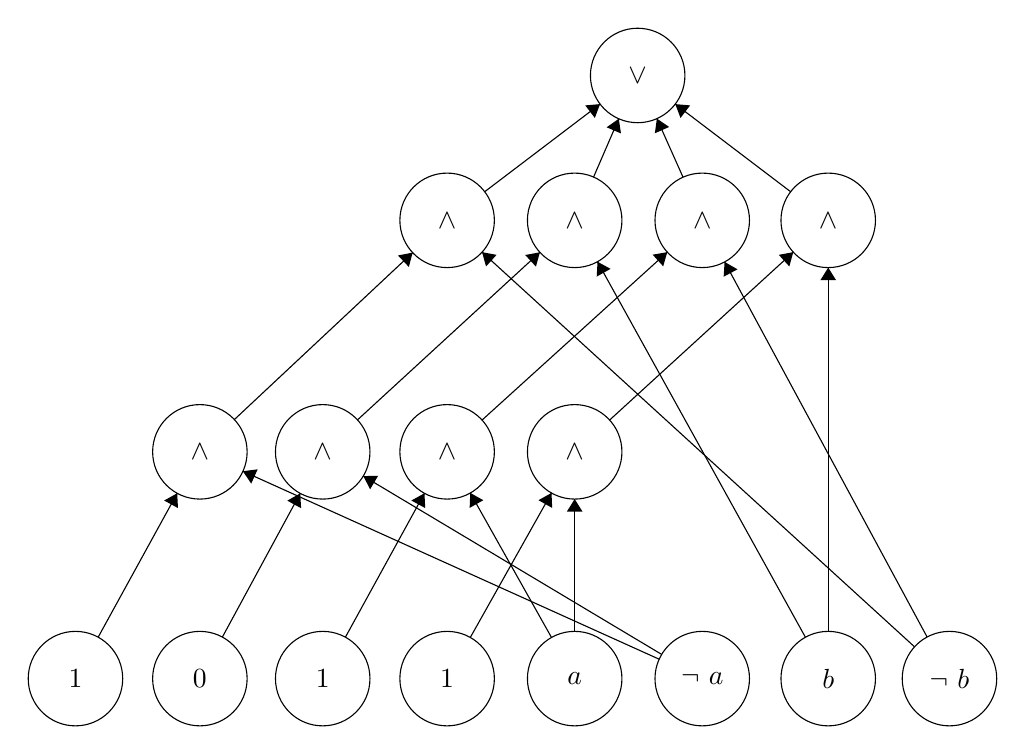
\begin{tikzpicture}[scale=0.2]
  \tikzstyle{every node}+=[inner sep=0pt]
  \draw [black] (6.4,-42.4) circle (3);
  \draw (6.4,-42.4) node {$1$};
  \draw [black] (14.3,-42.4) circle (3);
  \draw (14.3,-42.4) node {$0$};
  \draw [black] (22.1,-42.4) circle (3);
  \draw (22.1,-42.4) node {$1$};
  \draw [black] (30,-42.4) circle (3);
  \draw (30,-42.4) node {$1$};
  \draw [black] (38.1,-42.4) circle (3);
  \draw (38.1,-42.4) node {$a$};
  \draw [black] (46.2,-42.4) circle (3);
  \draw (46.2,-42.4) node {$\lnot\mbox{ }a$};
  \draw [black] (54.2,-42.4) circle (3);
  \draw (54.2,-42.4) node {$b$};
  \draw [black] (61.9,-42.4) circle (3);
  \draw (61.9,-42.4) node {$\lnot\mbox{ }b$};
  \draw [black] (14.3,-28) circle (3);
  \draw (14.3,-28) node {$\land$};
  \draw [black] (22.1,-28) circle (3);
  \draw (22.1,-28) node {$\land$};
  \draw [black] (30,-28) circle (3);
  \draw (30,-28) node {$\land$};
  \draw [black] (38.1,-28) circle (3);
  \draw (38.1,-28) node {$\land$};
  \draw [black] (30,-13.3) circle (3);
  \draw (30,-13.3) node {$\land$};
  \draw [black] (38.1,-13.3) circle (3);
  \draw (38.1,-13.3) node {$\land$};
  \draw [black] (46.2,-13.3) circle (3);
  \draw (46.2,-13.3) node {$\land$};
  \draw [black] (54.2,-13.3) circle (3);
  \draw (54.2,-13.3) node {$\land$};
  \draw [black] (42.1,-4.1) circle (3);
  \draw (42.1,-4.1) node {$\lor$};
  \draw [black] (7.84,-39.77) -- (12.86,-30.63);
  \fill [black] (12.86,-30.63) -- (12.03,-31.09) -- (12.91,-31.57);
  \draw [black] (43.47,-41.17) -- (17.03,-29.23);
  \fill [black] (17.03,-29.23) -- (17.56,-30.02) -- (17.97,-29.11);
  \draw [black] (15.73,-39.76) -- (20.67,-30.64);
  \fill [black] (20.67,-30.64) -- (19.85,-31.1) -- (20.73,-31.58);
  \draw [black] (23.54,-39.77) -- (28.56,-30.63);
  \fill [black] (28.56,-30.63) -- (27.73,-31.09) -- (28.61,-31.57);
  \draw [black] (31.47,-39.79) -- (36.63,-30.61);
  \fill [black] (36.63,-30.61) -- (35.8,-31.07) -- (36.67,-31.56);
  \draw [black] (43.62,-40.86) -- (24.68,-29.54);
  \fill [black] (24.68,-29.54) -- (25.11,-30.38) -- (25.62,-29.52);
  \draw [black] (36.63,-39.79) -- (31.47,-30.61);
  \fill [black] (31.47,-30.61) -- (31.43,-31.56) -- (32.3,-31.07);
  \draw [black] (38.1,-39.4) -- (38.1,-31);
  \fill [black] (38.1,-31) -- (37.6,-31.8) -- (38.6,-31.8);
  \draw [black] (16.49,-25.95) -- (27.81,-15.35);
  \fill [black] (27.81,-15.35) -- (26.88,-15.53) -- (27.57,-16.26);
  \draw [black] (24.31,-25.97) -- (35.89,-15.33);
  \fill [black] (35.89,-15.33) -- (34.96,-15.5) -- (35.64,-16.24);
  \draw [black] (32.22,-25.98) -- (43.98,-15.32);
  \fill [black] (43.98,-15.32) -- (43.05,-15.48) -- (43.72,-16.22);
  \draw [black] (40.32,-25.98) -- (51.98,-15.32);
  \fill [black] (51.98,-15.32) -- (51.06,-15.49) -- (51.73,-16.23);
  \draw [black] (59.68,-40.38) -- (32.22,-15.32);
  \fill [black] (32.22,-15.32) -- (32.47,-16.23) -- (33.14,-15.49);
  \draw [black] (60.48,-39.76) -- (47.62,-15.94);
  \fill [black] (47.62,-15.94) -- (47.56,-16.88) -- (48.44,-16.41);
  \draw [black] (52.75,-39.77) -- (39.55,-15.93);
  \fill [black] (39.55,-15.93) -- (39.5,-16.87) -- (40.38,-16.38);
  \draw [black] (54.2,-39.4) -- (54.2,-16.3);
  \fill [black] (54.2,-16.3) -- (53.7,-17.1) -- (54.7,-17.1);
  \draw [black] (32.39,-11.48) -- (39.71,-5.92);
  \fill [black] (39.71,-5.92) -- (38.77,-6) -- (39.38,-6.8);
  \draw [black] (39.3,-10.55) -- (40.9,-6.85);
  \fill [black] (40.9,-6.85) -- (40.13,-7.39) -- (41.04,-7.78);
  \draw [black] (44.98,-10.56) -- (43.32,-6.84);
  \fill [black] (43.32,-6.84) -- (43.19,-7.77) -- (44.1,-7.37);
  \draw [black] (51.81,-11.48) -- (44.49,-5.92);
  \fill [black] (44.49,-5.92) -- (44.82,-6.8) -- (45.43,-6);
  \end{tikzpicture}
  \caption{Circuit for retrieving an item from a database with four elements.}
  \label{fig:fig1}  
\end{figure}
Now, we describe an approach for such evaluations on ciphertexts. The approach below originally comes from the GSW scheme from~\cite{gsw13}, but of course this is not the only scheme that would work. Our goal is to explain that such approaches can be natural and interesting not just in a theoretical setting.

Further, we observe that fully homomorphic encryption is not necessary for our purposes, which in turn should allow much more practical concrete applications.

\subsection{Definitions}



\bibliographystyle{unsrt}
\bibliography{refs}

\end{document}